\documentclass{beamer}
\usetheme{Boadilla}
\usecolortheme{beaver}

\usepackage{forest}
\usepackage{tikz-qtree}
\begin{document}

\title{Extracting Syntactic Trees from NMT Encoder Self-Attentions}
%\subtitle{NPFL097}
\author[D. Mare\v{c}ek, R. Rosa]{\textbf{David Mare\v{c}ek}, Rudolf Rosa}
\institute[]{Institute of Formal and Applied Linguistics, Charles University, Prague \\\bigskip BlackboxNLP Workshop, EMNLP, Brussels}
\date{November 1st, 2018} 

%--- the titlepage frame -------------------------%
\begin{frame}[plain]
  \titlepage
\end{frame}

%\begin{frame}{Machine Translation in 2010}
%    TectoMT system (Popel et al. 2010)
%    \begin{center}
%    \includegraphics[scale=0.2]{tectomt.png}
%    \end{center}
%\end{frame}
%
%\begin{frame}{Machine Translation in 2010}
%    %TectoMT system
%    \begin{center}
%    English $\rightarrow$ Czech
%
%    \bigskip
%    \textbf{BLEU: 13.9}
%    \end{center}
%\end{frame}

\begin{frame}{Current state of the art in Machine Translation}
    \begin{columns}
        \column{0.5\textwidth}
    	    Neural Machine Translation
            \bigskip

            \begin{itemize}
                \item e.g. the Transformer architecture (Vaswani et al. 2017)
                \item translation quality comarable with human translators (WMT18 news-translation shared taks)
            \end{itemize}
        \column{0.5\textwidth}
        \begin{center}
            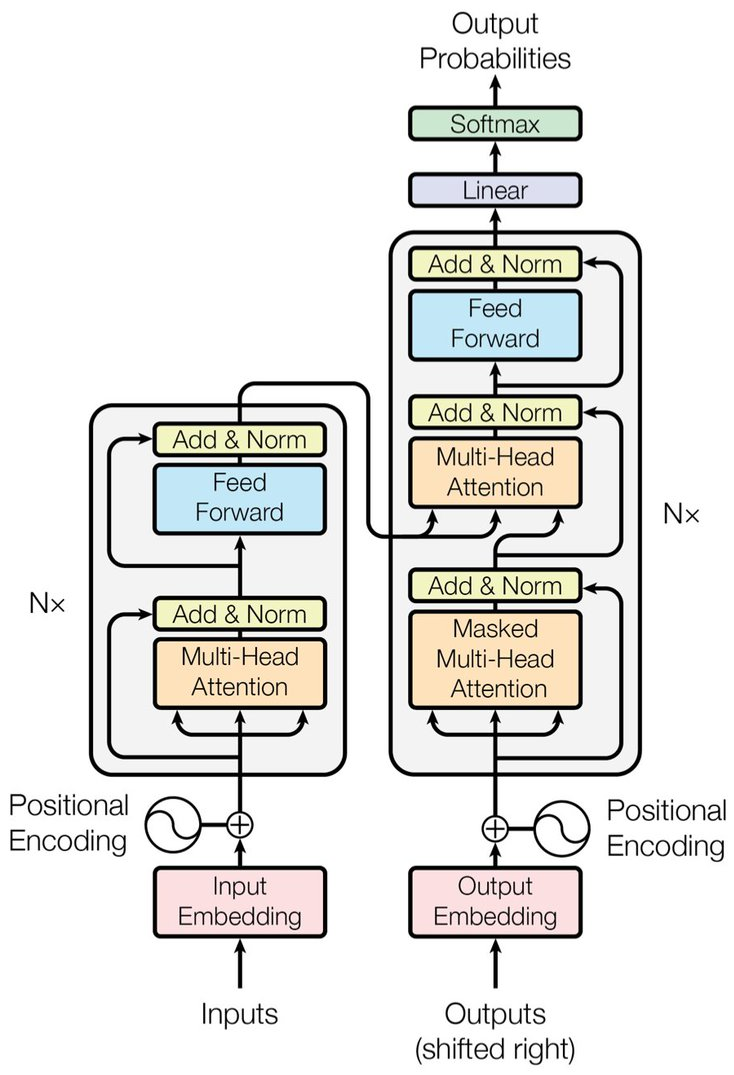
\includegraphics[scale=0.17]{transformer.png}
        \end{center}
    \end{columns}
\end{frame}

%\begin{frame}{Current state of the art in Machine Translation}
%    \begin{center}
%    English $\rightarrow$ Czech
%    \bigskip
%    \textbf{BLEU: 26.8}
%    \end{center}
%\end{frame}

\begin{frame}{Is there any latent syntax learned inside?}
    %\begin{center}
    %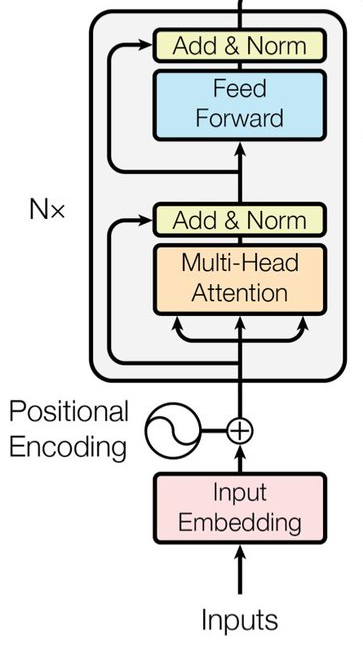
\includegraphics[scale=0.3]{transformer-encoder.png}
    %\end{center}
    Current end-to-end NMT systems are very hard to interpret.
    \begin{itemize}
        \item plenty of high-dimensional vectors
        \item the self-attention mechanism mixes everything together
    \end{itemize}
    
    \bigskip
    Is there any latent syntax learned inside?

    \bigskip
    This work:
    \begin{itemize}
	\item Use state-of-the art NMT system (Transformer).
        \item Extract and analyze its encoder self-attentions.
        \item Based on the self-attentions, induce parse trees and compare them to manually annotated treebanks. 
    \end{itemize}
\end{frame}

%URRENT BEST METHODS
% FOR MACHINE TRANSLATION
%  DO NOT USE ANY
%   LINGUISTIC ANNOTATIONS
%
%IS THERE ANY LANTENT SYNTAX 
%    LEARNED BY NEURAL
%        MACHINE TRANSLATION ???
%
%Use state-of-the art NMT system Transformer
%Extract and analyze encoder self-attentions
%Create parse trees using self-attentions matrices
%Compare it to manually annotated treebanks

%\begin{frame}{Transformer - Encoder}
%    \begin{columns}
%        \column{0.5\textwidth}
%            \begin{itemize}
%                \item For each position, the self-attention mechanism looks at all other positions in the previous layer
%                \item Residual connections boost the information about particular position from the previous layer
%                \item Attentions to the same positions are learned to be weaker because of these residual connections
%            \end{itemize}
%        \column{0.5\textwidth}
%        \begin{centering}
%        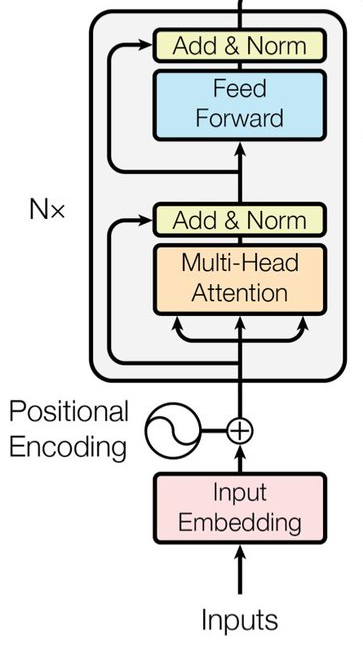
\includegraphics[scale=0.25]{transformer-encoder.png}
%        \end{centering}
%    \end{columns}
%\end{frame}

\begin{frame}{Self-Attention mechanism}
    \begin{itemize}
         \item For each position (source word), the self-attention mechanism can look at all positions in the previous layer
         \item Residual connections boost the attention to the same position in the previous layer
         \item Typically 16 heads, each with different weights
    \end{itemize}
    \bigskip
    \begin{center}
        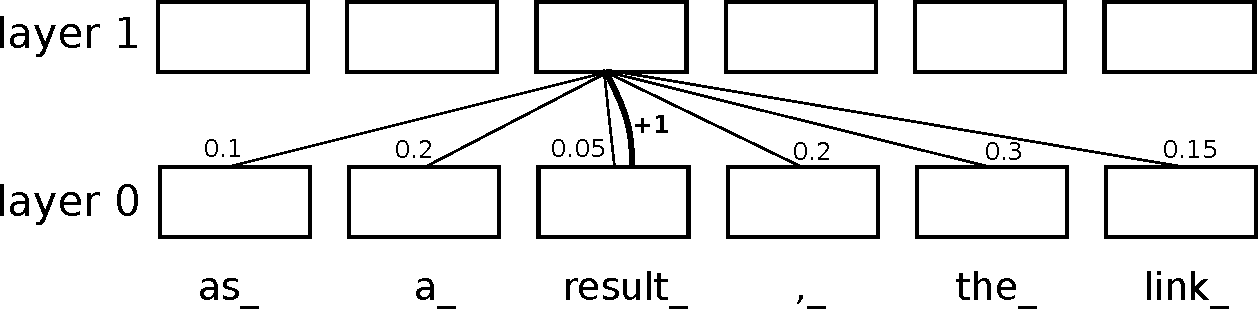
\includegraphics[scale=0.5]{attention.pdf}
    \end{center}
\end{frame}

\begin{frame}{Heads with syntactic properties}
    Original paper self-attention visualization (Vaswani, 2017):
    \begin{center}
    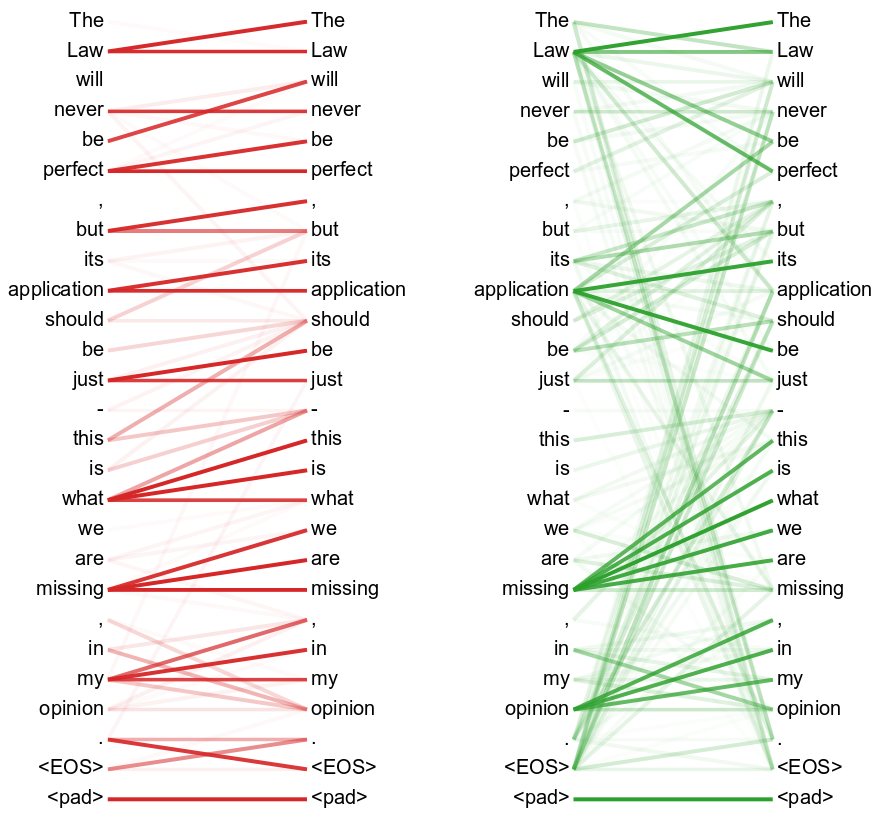
\includegraphics[scale=0.22]{vasw1.png}
    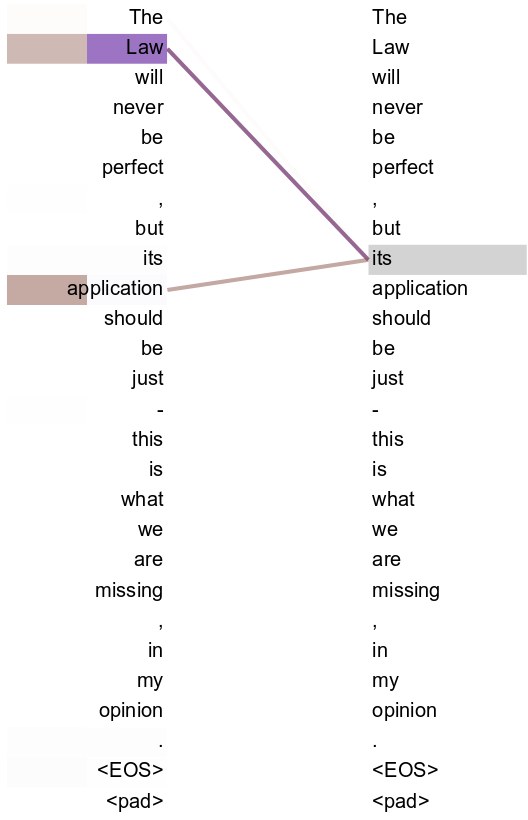
\includegraphics[scale=0.219]{vasw2.png}
    \end{center}
\end{frame}

\begin{frame}{Experiments}
    \begin{itemize}
        \item We trained Transformer in its standard setting (6 layers, 16 heads, ...)
        \item Europarl parallel corpus
        \begin{itemize}
            \item English$\rightarrow$Czech
            \item English$\rightarrow$German
            \item English$\rightarrow$French
            \item English$\rightarrow$Finnish
        \end{itemize}
        \item BPE, dictionary size 100k
        \item We translated 1000 test sentences and extract encoder self-attentions weights
    \end{itemize}
\end{frame}


\begin{frame}{Visualisation of one self-attention head}
    \begin{columns}
        \column{0.5\textwidth}
            \begin{itemize}
                \item square matrix
                \item each row shows attention distribution of one word across all the words in the previous layer
                \item attention to the same position (diagonal) is strong due to residual connections
                \item we have 6 layers x 16 heads = 96 heads in total
            \end{itemize}
        \column{0.5\textwidth}
        \begin{centering}
        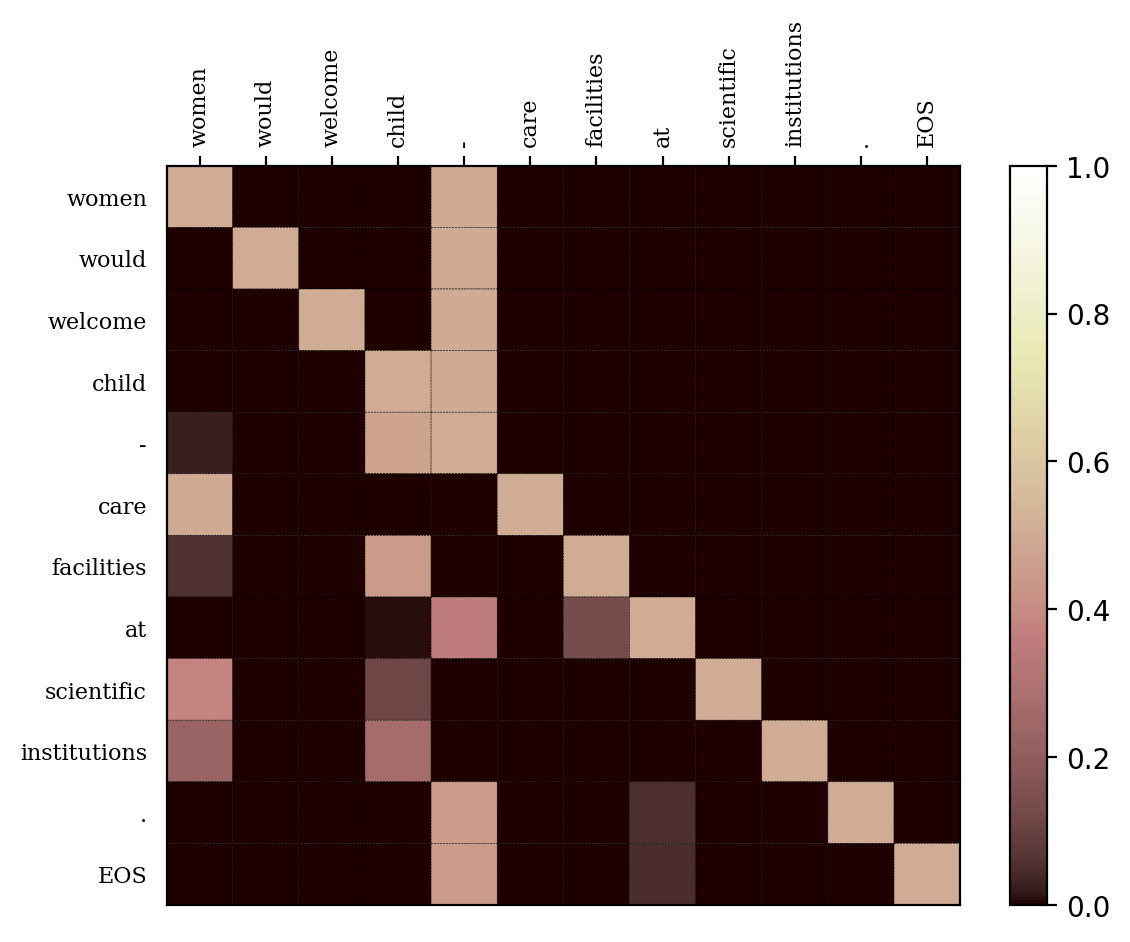
\includegraphics[scale=0.4]{more_complicated.png}
        \end{centering}
    \end{columns}
\end{frame}

\begin{frame}{Analysis of attention heads}
    \begin{itemize}
         \item $\sim$ 15\% of all heads (mainly in the first layer) look at the previous, at the same, or at the next word.
    \end{itemize}
    \begin{center}
        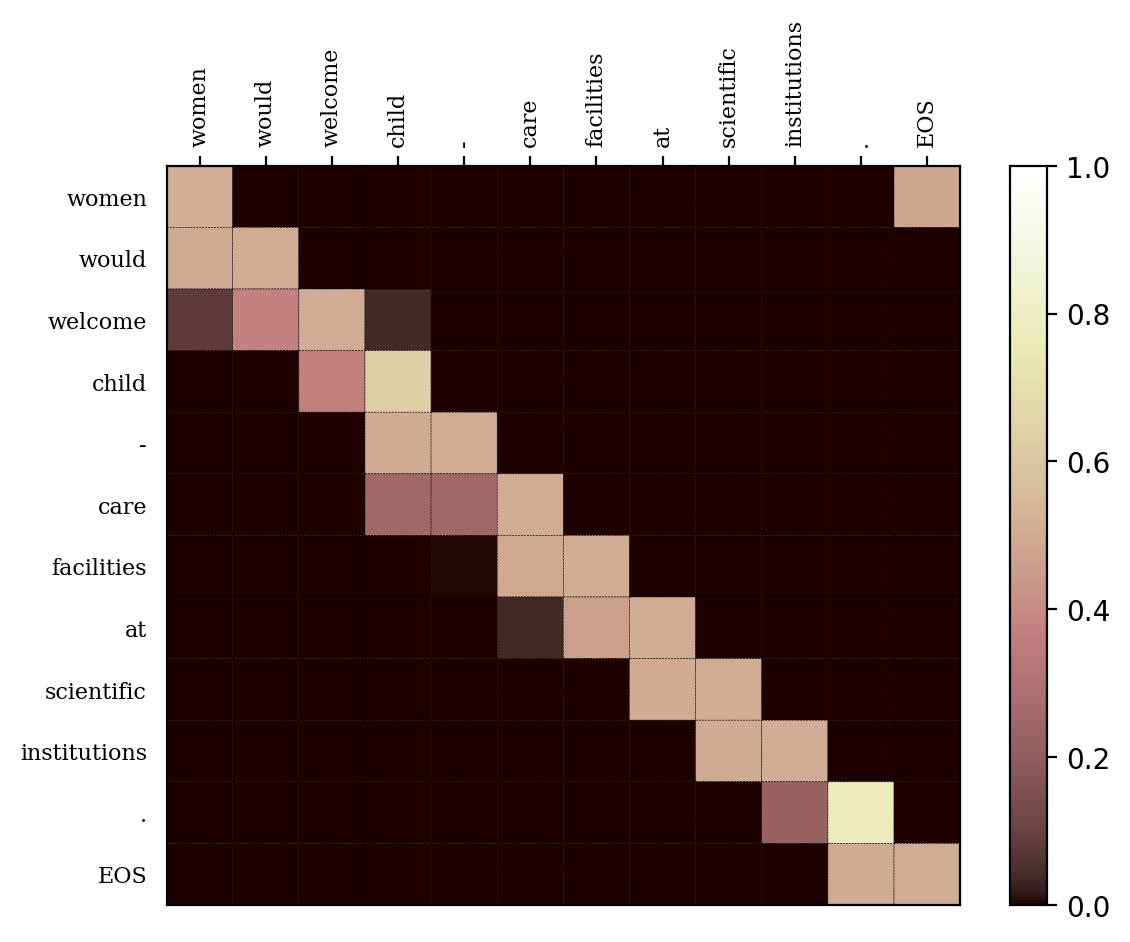
\includegraphics[scale=0.5]{look_at_previous.png}
    \end{center}
\end{frame}

\begin{frame}{Analysis of attention heads}
    \begin{itemize}
         \item $\sim$ 15\% of all heads form continuous phrases looking at their first word.
    \end{itemize}
    \begin{center}
        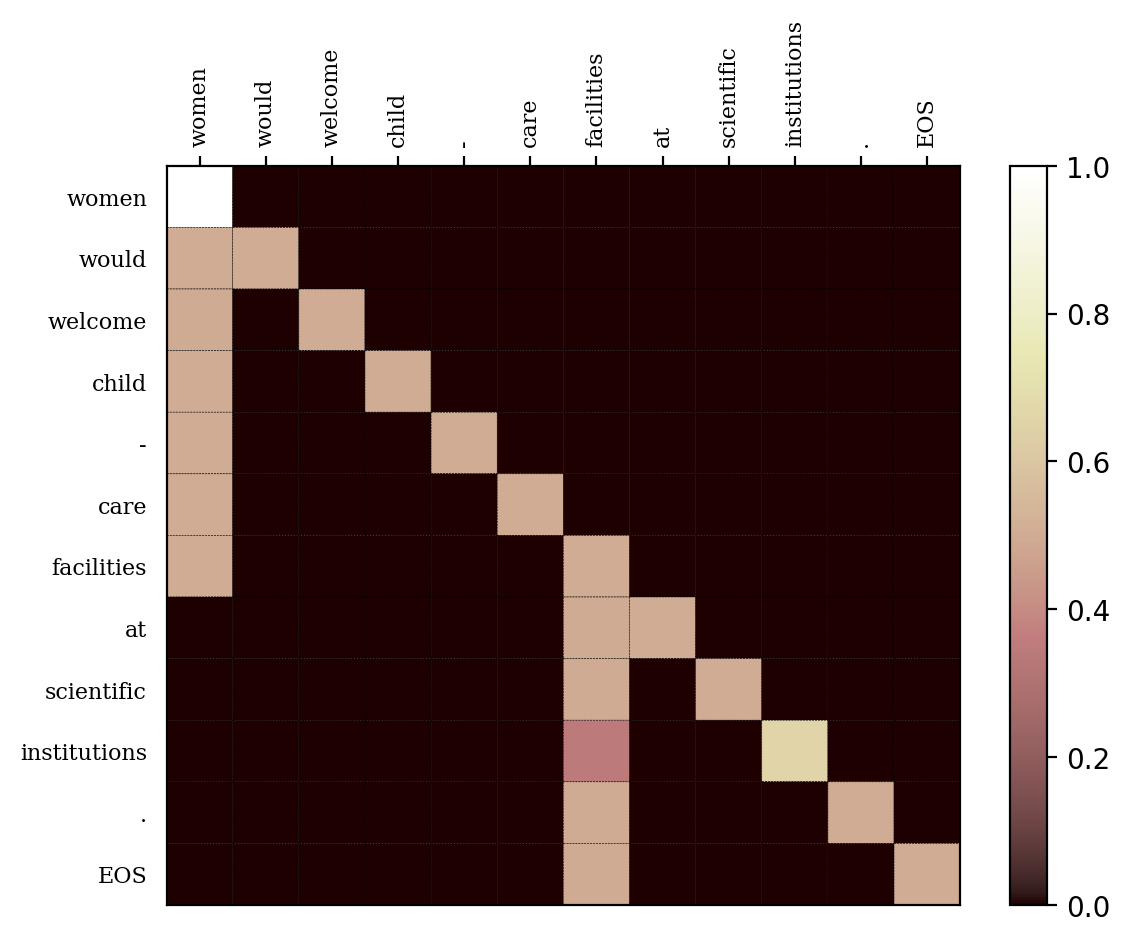
\includegraphics[scale=0.5]{look_at_first.png}
    \end{center}
\end{frame}

\begin{frame}{Analysis of attention heads}
    \begin{itemize}
         \item $\sim$ 15\% of all heads form continuous phrases looking at their last word.
    \end{itemize}
    \begin{center}
        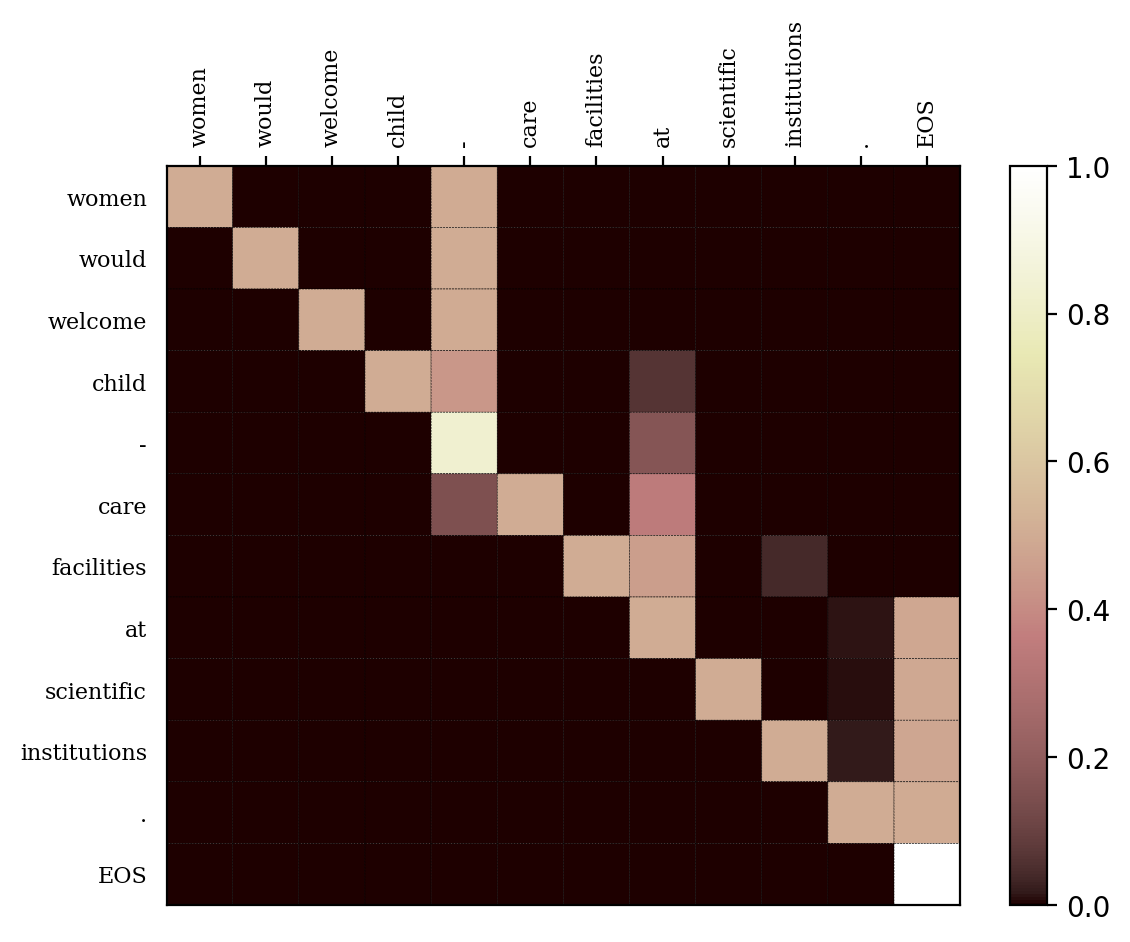
\includegraphics[scale=0.5]{look_at_last.png}
    \end{center}
\end{frame}

\begin{frame}{Analysis of attention heads}
    \begin{itemize}
         \item $\sim$ 20\% of all heads form continuous phrases looking at another word.
    \end{itemize}
    \begin{center}
        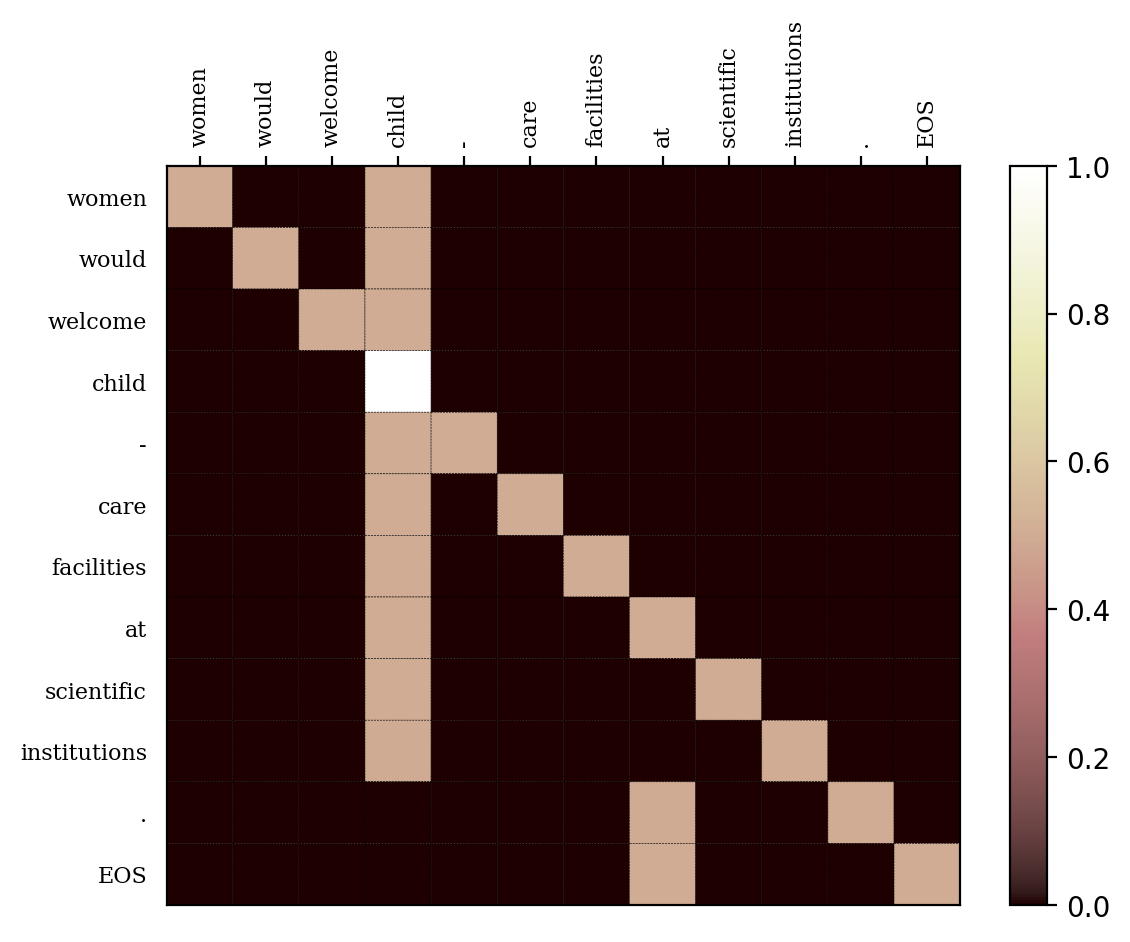
\includegraphics[scale=0.5]{look_at_another.png}
    \end{center}
\end{frame}

\begin{frame}{Analysis of attention heads}
    \begin{itemize}
         \item In $\sim$ 5\% of all heads, all the words look at the end of the sentence.
    \end{itemize}
    \begin{center}
        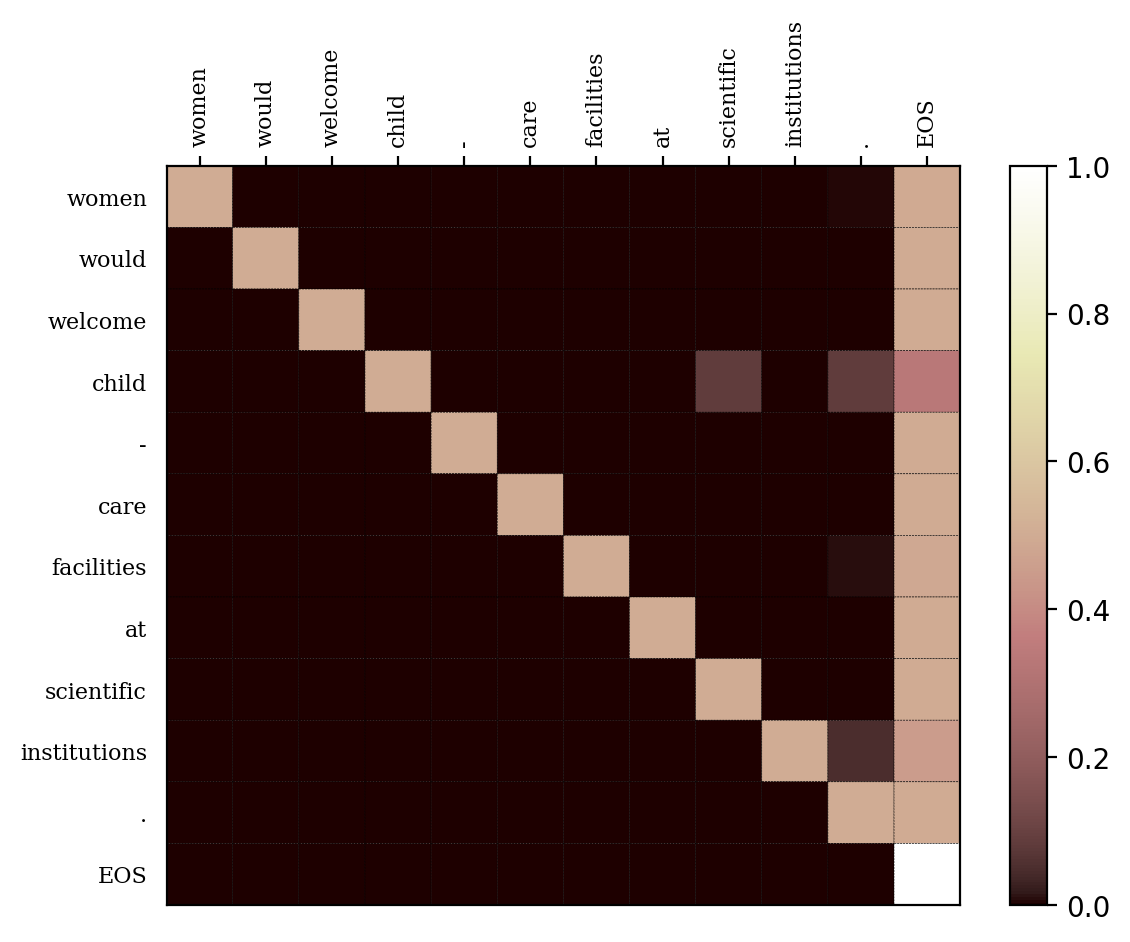
\includegraphics[scale=0.5]{look_at_eos.png}
    \end{center}
\end{frame}

\begin{frame}{Analysis of attention heads}
    \begin{itemize}
         \item Rest $\sim$ 30\% of heads are more complicated.
    \end{itemize}
    \begin{center}
        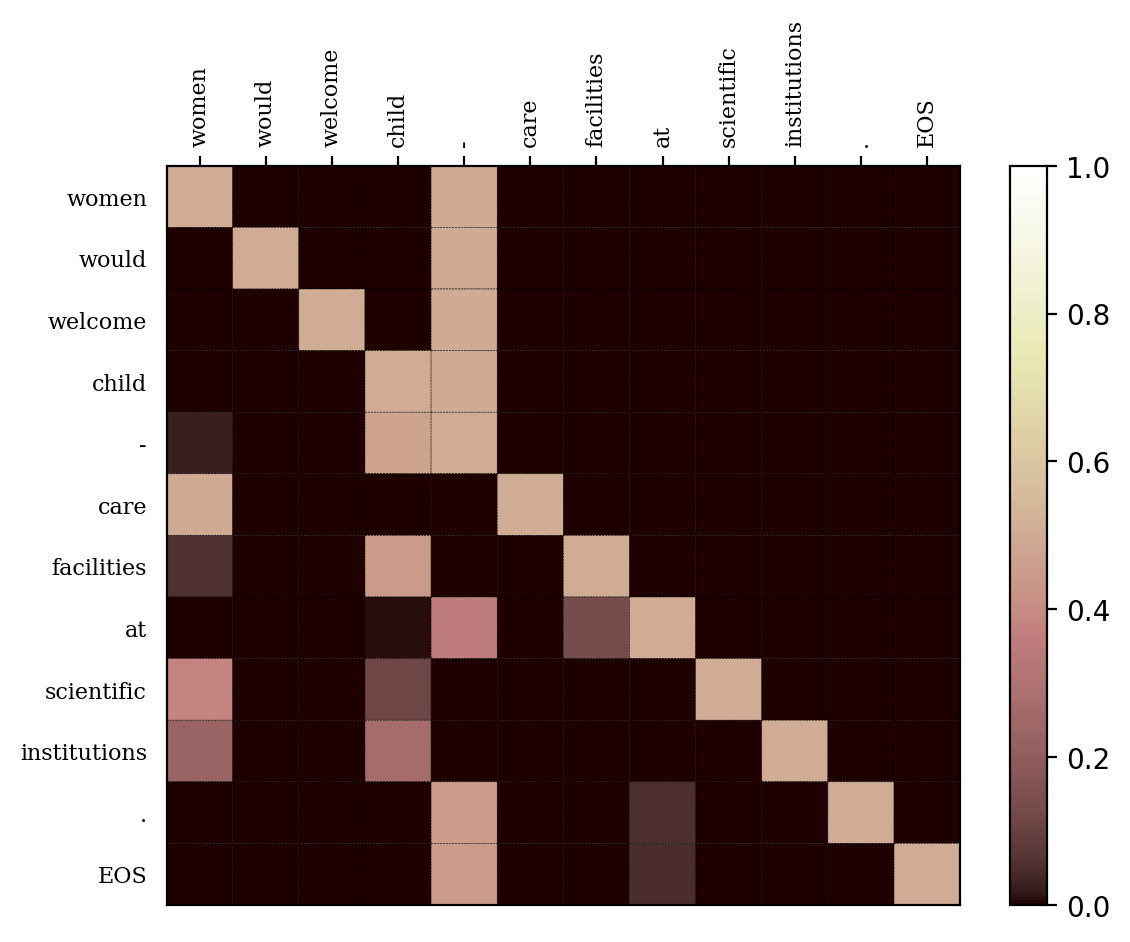
\includegraphics[scale=0.5]{more_complicated.png}
    \end{center}
\end{frame}

\begin{frame}{From self-attentions to trees}
\begin{itemize}
    %\item So far we \textbf{do not select} heads that are ``more syntactic''
    \item We know that majority of heads form ``continuous phrases''. 
    \item We collect all such continuous phrases \textbf{across all the heads and layers} in the encoder.
    \item For each possible phrase, we compute its score reflecting its frequency.
\end{itemize}
   \begin{center}
        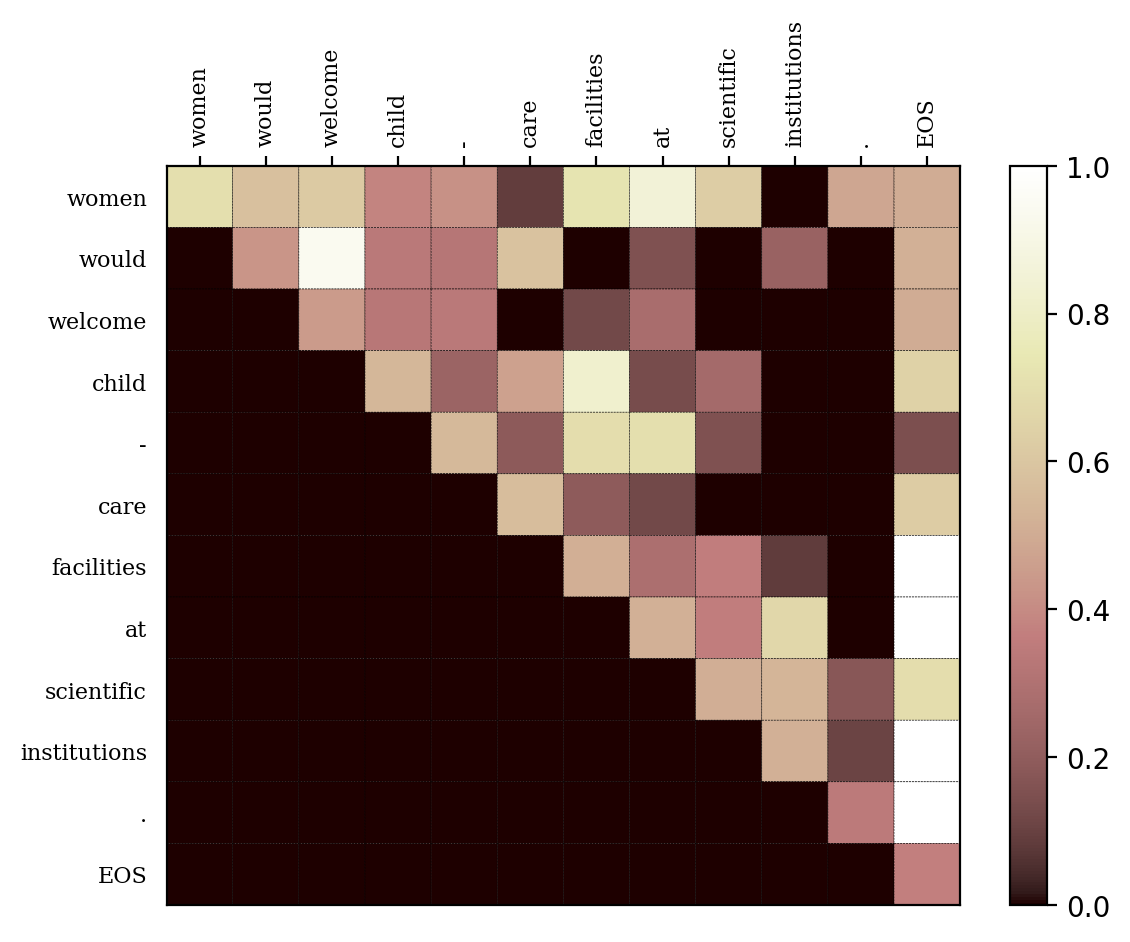
\includegraphics[scale=0.43]{weights-s5.png}
        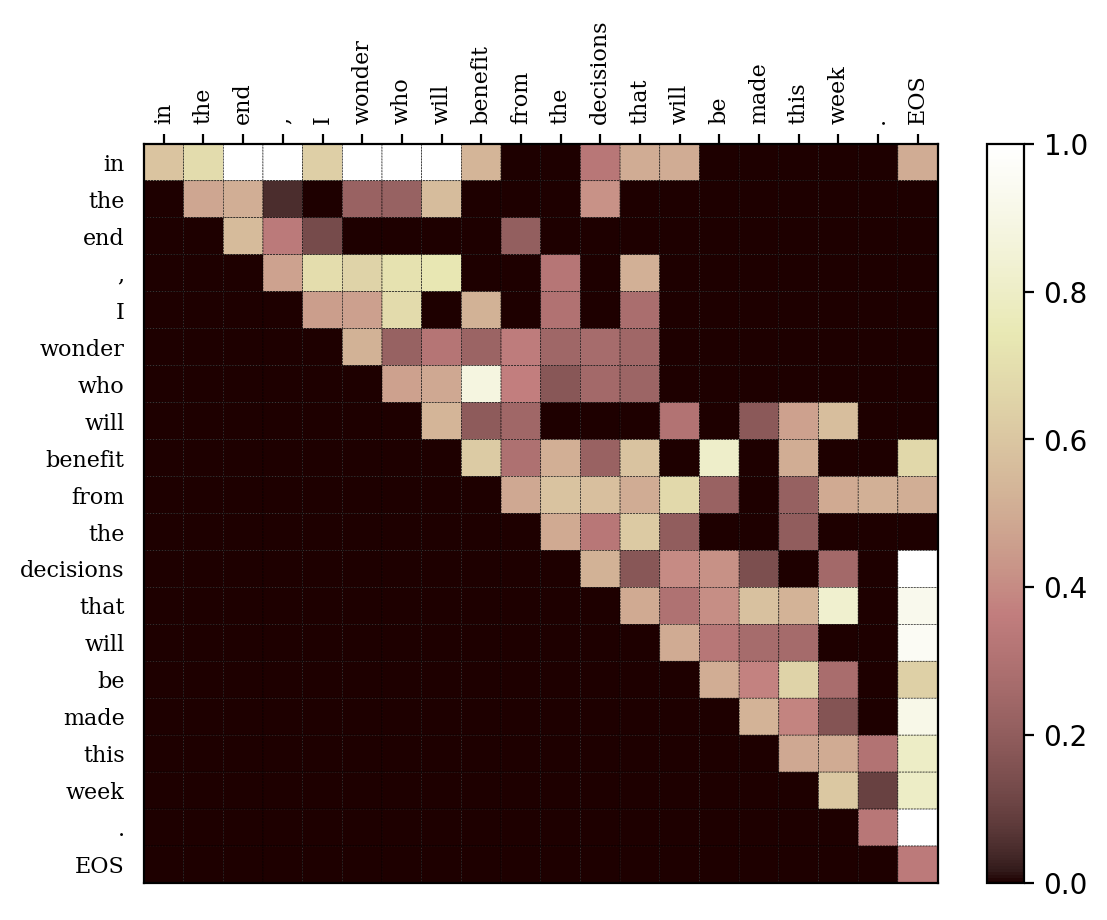
\includegraphics[scale=0.43]{weights-s25.png}
    \end{center}
\end{frame}

%\begin{frame}{analysis = correctly distinguished phenomena}
%clauses
%\end{frame}

\begin{frame}{Constituency parsing using CKY}
    \begin{itemize}
        \item We find the best phrase-tree (comprising the best scoring phrases) using CKY algorithm.
        \item Probability of joining two phrases together and probability of the two respective subtrees is weighted 1:1
    \end{itemize}
    \begin{center}
        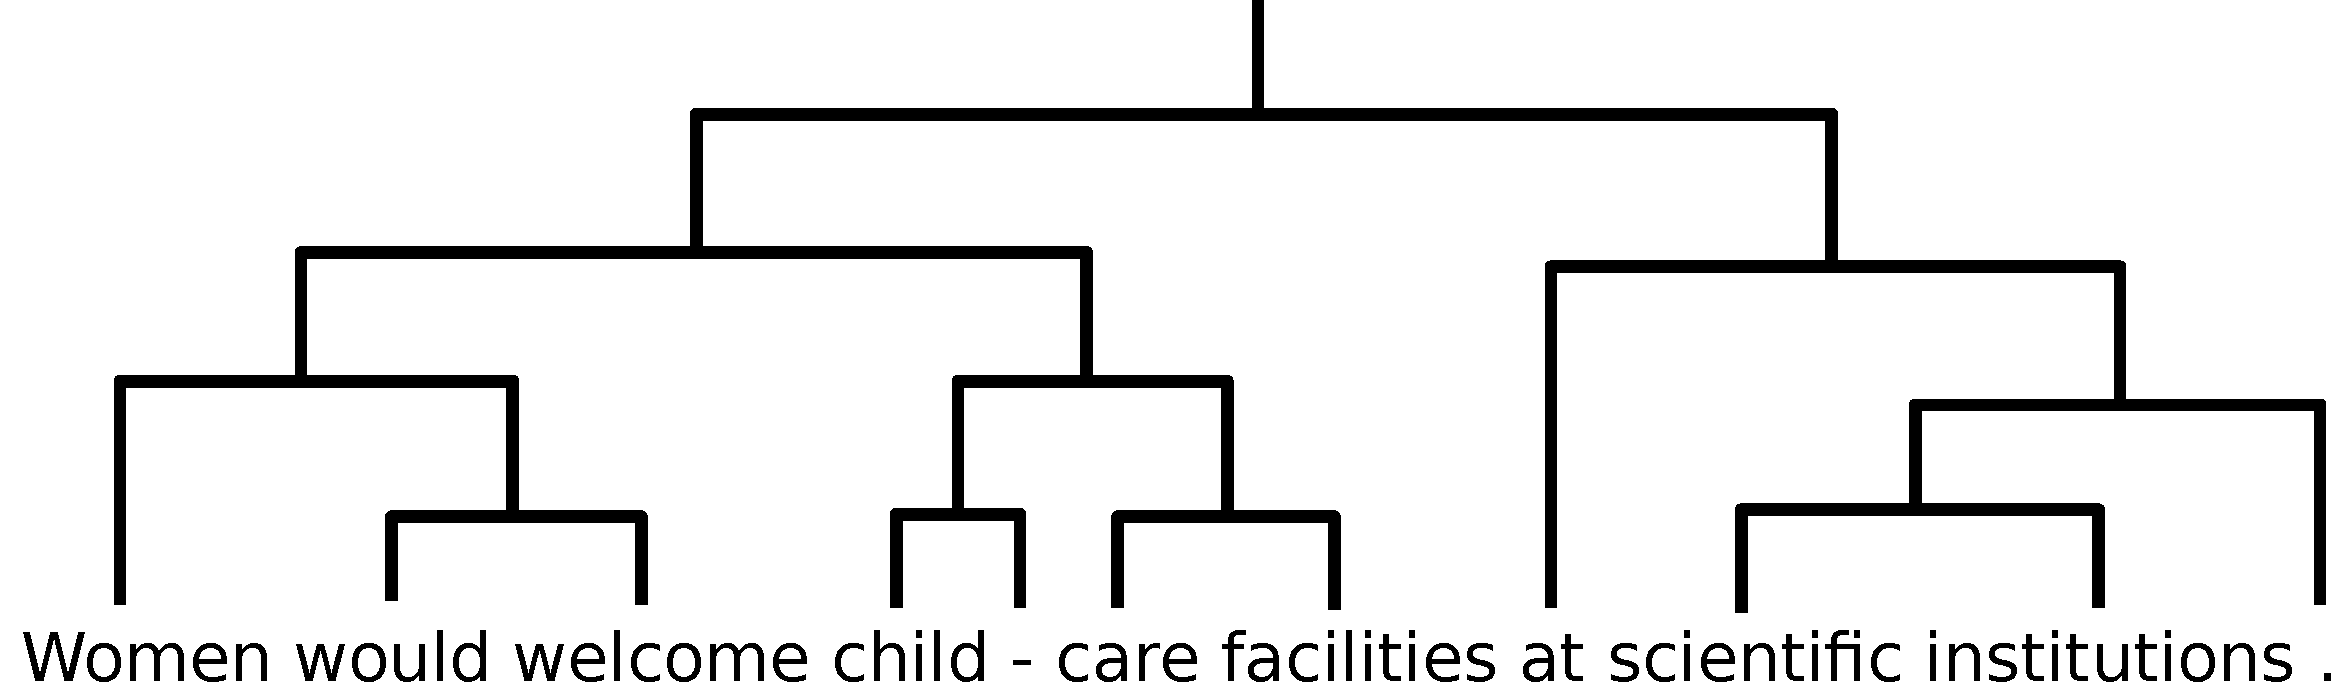
\includegraphics[scale=0.3]{tree.pdf}
    \end{center}
\end{frame}


\begin{frame}{Evaluation}
\begin{enumerate}
    \item Against Stanford parser trained on Penn Treebank
    \begin{itemize}
        \item compute precision, recall, and F1 score on individual brackets
    \end{itemize}
    \item Against UDPipe parser trained on UniversalDependencies English treebank
    \begin{itemize}
        \item convert dependency structures into phrase structures
        \item compute the ratio of valid (non-crossing) brackets
        \item compute precision, recall, F1 score
        \item recall is very high since the phrase trees converted from dependency trees are very flat
    \end{itemize}
\end{enumerate}
\end{frame}

%\begin{frame}{Evaluation Baselines}
%\begin{itemize}
%    \item left binary branching
%    \item right binary branching
%    \item ballanced binary branching from left
%    \item ballanced binary branching from right
%\end{itemize}
%\end{frame}
 

\begin{frame}{Results}
\textbf{F1 scores}
\bigskip

\begin{centering}
\begin{tabular}{lrr}
method                 & Stanford PTB & Universal Dependencies \\
\hline
EN left branching      & 11.1\% & 37.4\%\\
EN right branching     & 12.1\% & 38.5\%\\
EN left ballanced      & 22.0\% & 56.1\%\\
EN right ballanced     & 26.4\% & 58.8\%\\
\hline
EN-CS self-attentions  & 30.9\% & 63.8\%\\
EN-DE self-attentions  & 30.3\% & 62.8\%\\
EN-FR self-attentions  & 28.4\% & 60.8\%\\
EN-FI self-attentions  & 30.6\% & 64.8\%\\
\end{tabular}
\end{centering}
\end{frame}

\begin{frame}{Conclusions}
We found that:
\begin{itemize}
    \item In a majority of attention heads, the whole continuous phrases look at the same word in the previous layer.
    \item The phrases are often in agreement with the linguistic theories.
    \item If we extract such phrases and build a constituency tree, it is better than left/right branching and ballanced binary baselines.
    \item The encoder very well separates longer sentences into clauses. It easily finds commas and conjunctions.
\end{itemize}
Some kind of syntax is probably learned, but is quite different for the one annotated in treebanks.
\end{frame}

\begin{frame}{Conclusions}
    \begin{center}
    \textbf{Thank you for your attention!}
    \end{center}
\end{frame}

\end{document}
